Powered wheelchairs have enabled greater independence for people with disability.
However, the use of this technology can be inaccessible or unsafe for people
with amyotrophic lateral sclerosis (ALS) or vision impairment,
who may be unable to use a joystick or see their environment clearly.

\subsection{Aims}
This research aims to develop a semi-autonomous smart wheelchair system.
This research is done in collaboration with Glide, a WA wheelchair manufacturer,
who have provided an existing powered wheelchair (CentroGlide) to use as a base
for this functionality (\cref{fig:wheelchair}). By developing assistive technology for the wheelchair,
the user is granted greater mobility, confidence, and independence.

\begin{figure}[H]
    \centering
    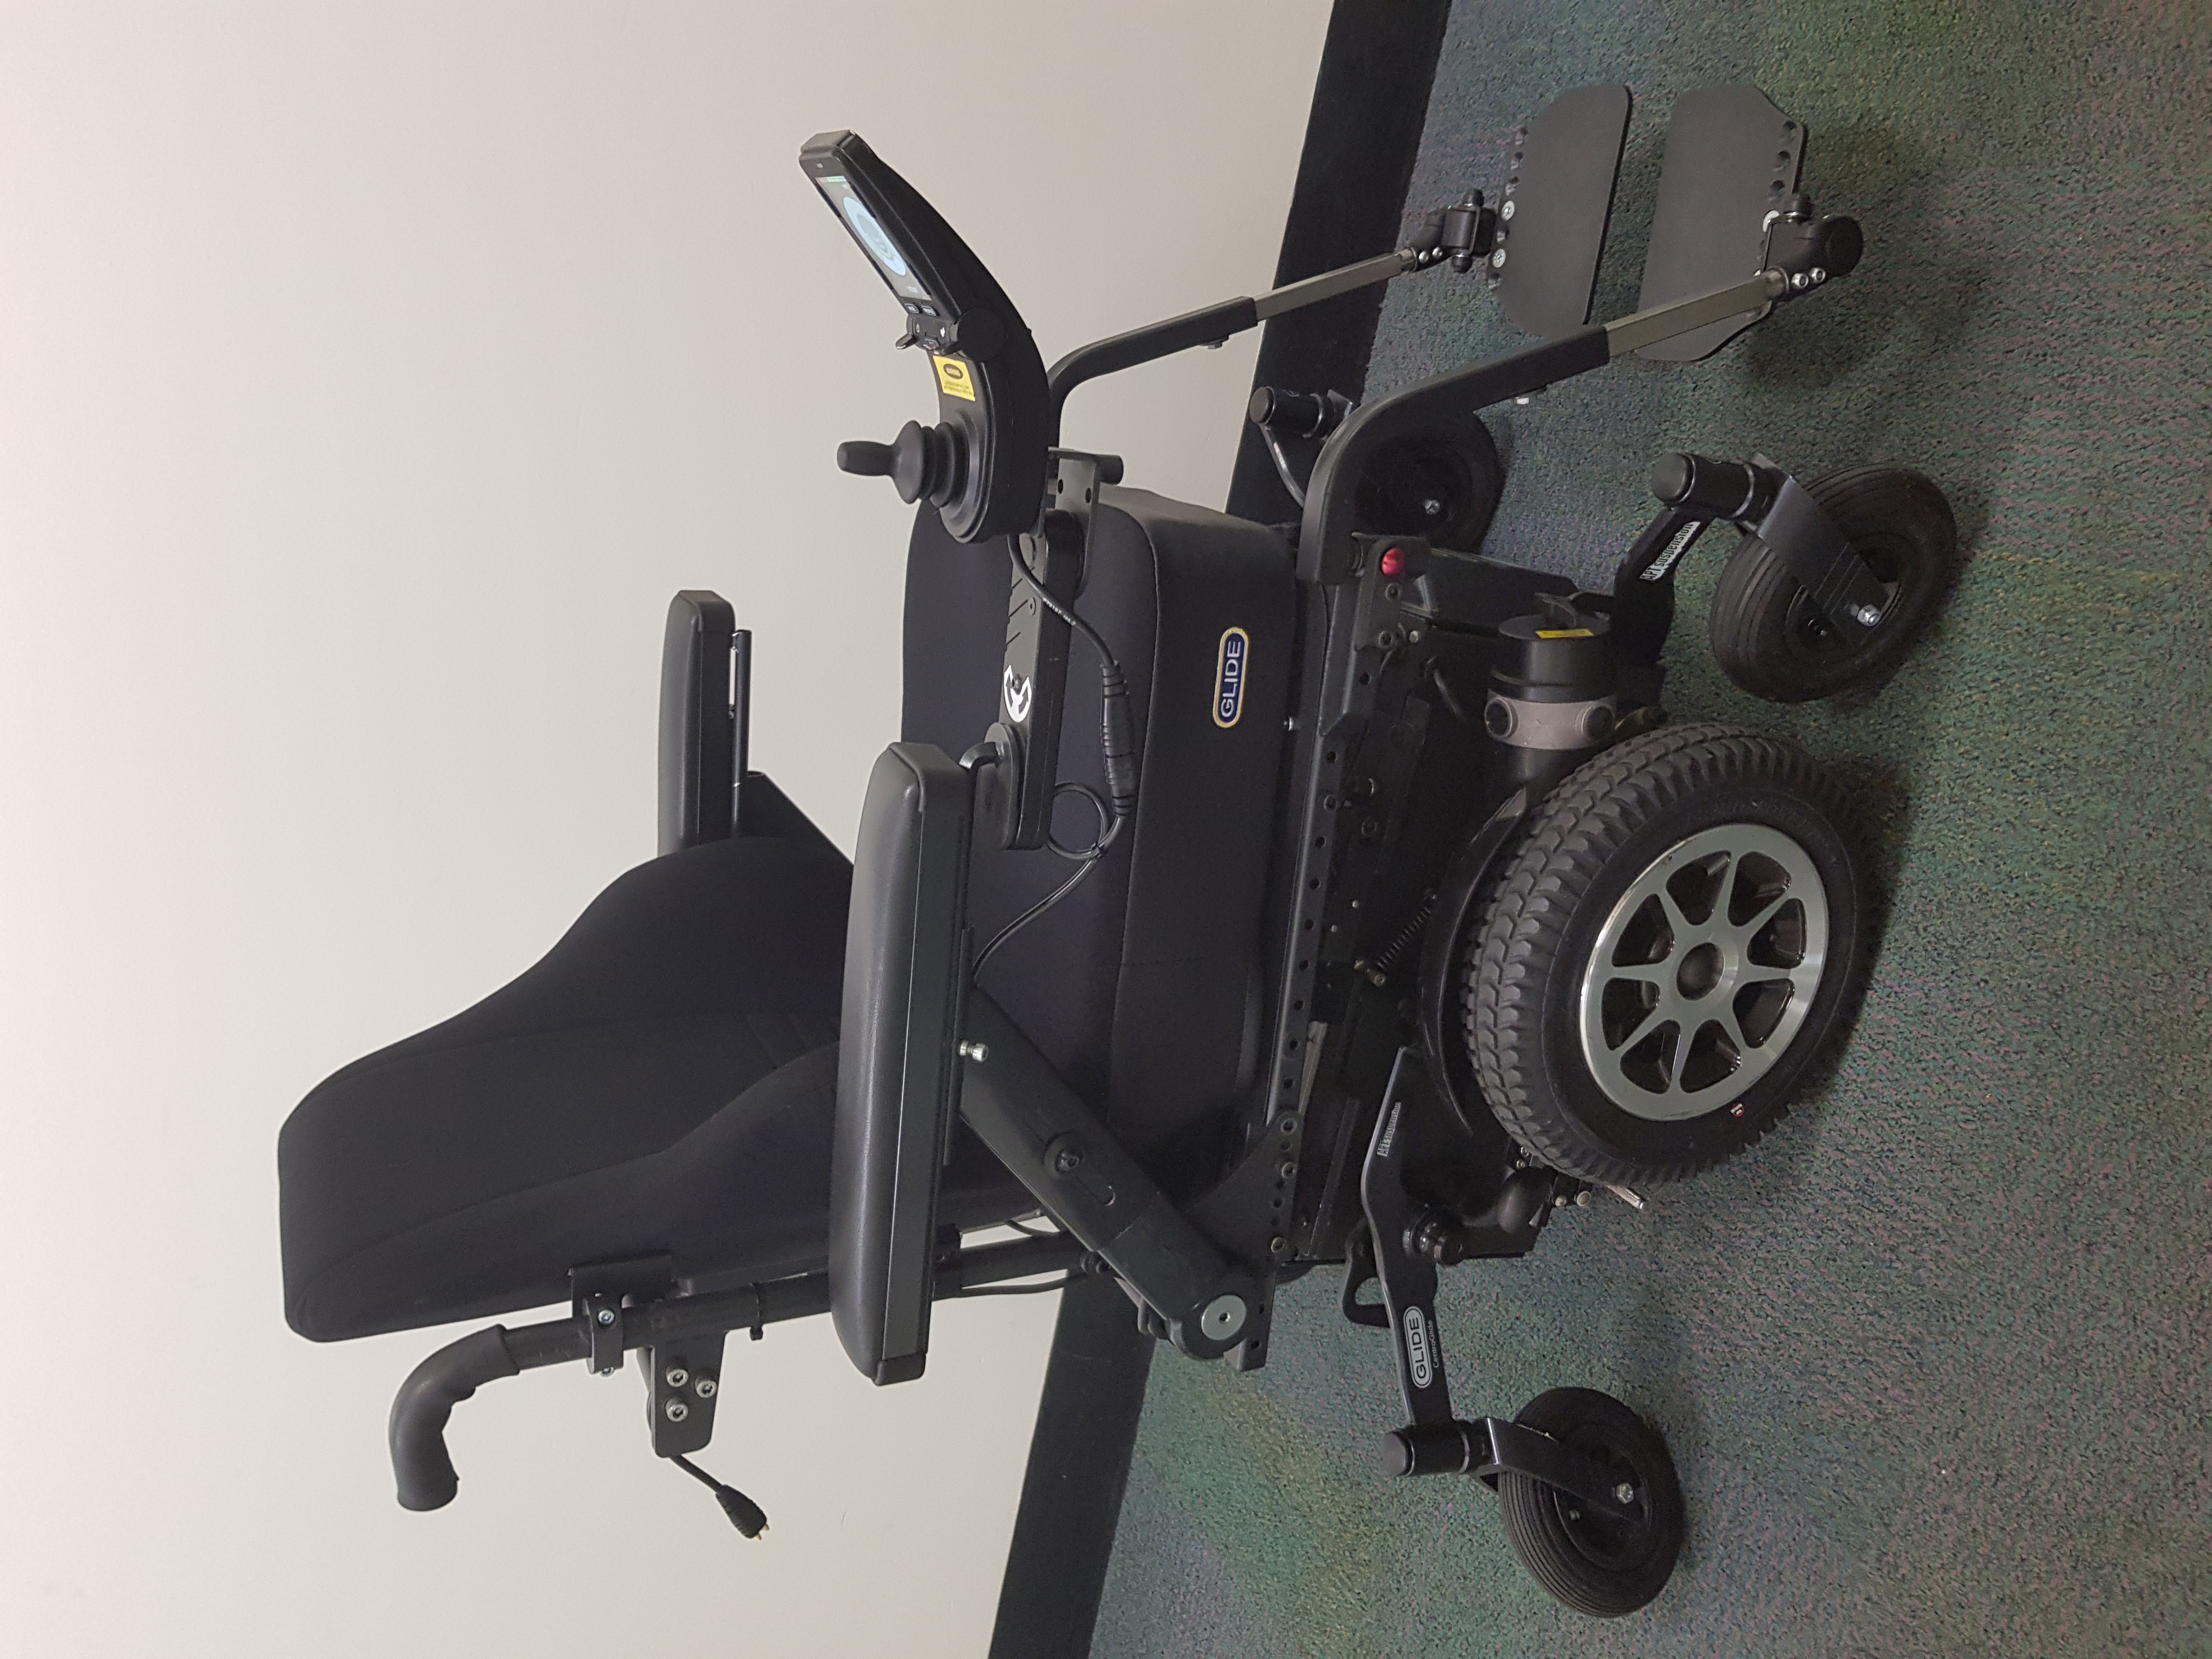
\includegraphics[width=0.55\linewidth,angle=270,origin=c]{images/wheelchair.jpg}
    \caption{The CentroGlide wheelchair}
    \label{fig:wheelchair}
\end{figure}

\pagebreak
\subsection{Problem Definition}
Multiple engineering project students are part of this team
and are working on elements such as controller design, navigation assistance, and object detection.
This work specifically focuses on pathway assistance, which identifies suitable
paths for the wheelchair to drive on. If a user unintentionally drives off their desired path,
this can lead to uneven terrain and possibly falling from the wheelchair.
By guiding the user along a path, these safety issues can be mitigated.

Emphasis is placed on the 'semi-autonomous' aspect of the wheelchair.
An important requirement of this project is that the user still
has control over their wheelchair, and can override any autonomous functionality
if required. If the smart wheelchair system mistakenly detects an obstacle,
the user's mobility should not be compromised.

Another requirement of the system is that any sensors mounted to the wheelchair
should not impede the user's comfort or the wheelchair's manoeuvrability.
Many wheelchair users have specific requirements for wheelchair seat adjustments,
to avoid pressure sores and discomfort. \Cref{fig:wheelchair_reclined} shows the
wheelchair configuration when fully reclined, demonstrating that some sensor mounting locations
are infeasible.

The smart wheelchair system should also be commercially viable - high-cost
components and sensors are infeasible. Internet connectivity should not be a requirement
for the system to operate either - the round trip time required to communicate with a server
could compromise the safety of a user. Because of this, all processing is performed locally
on the wheelchair.

\begin{figure}[H]
    \centering
    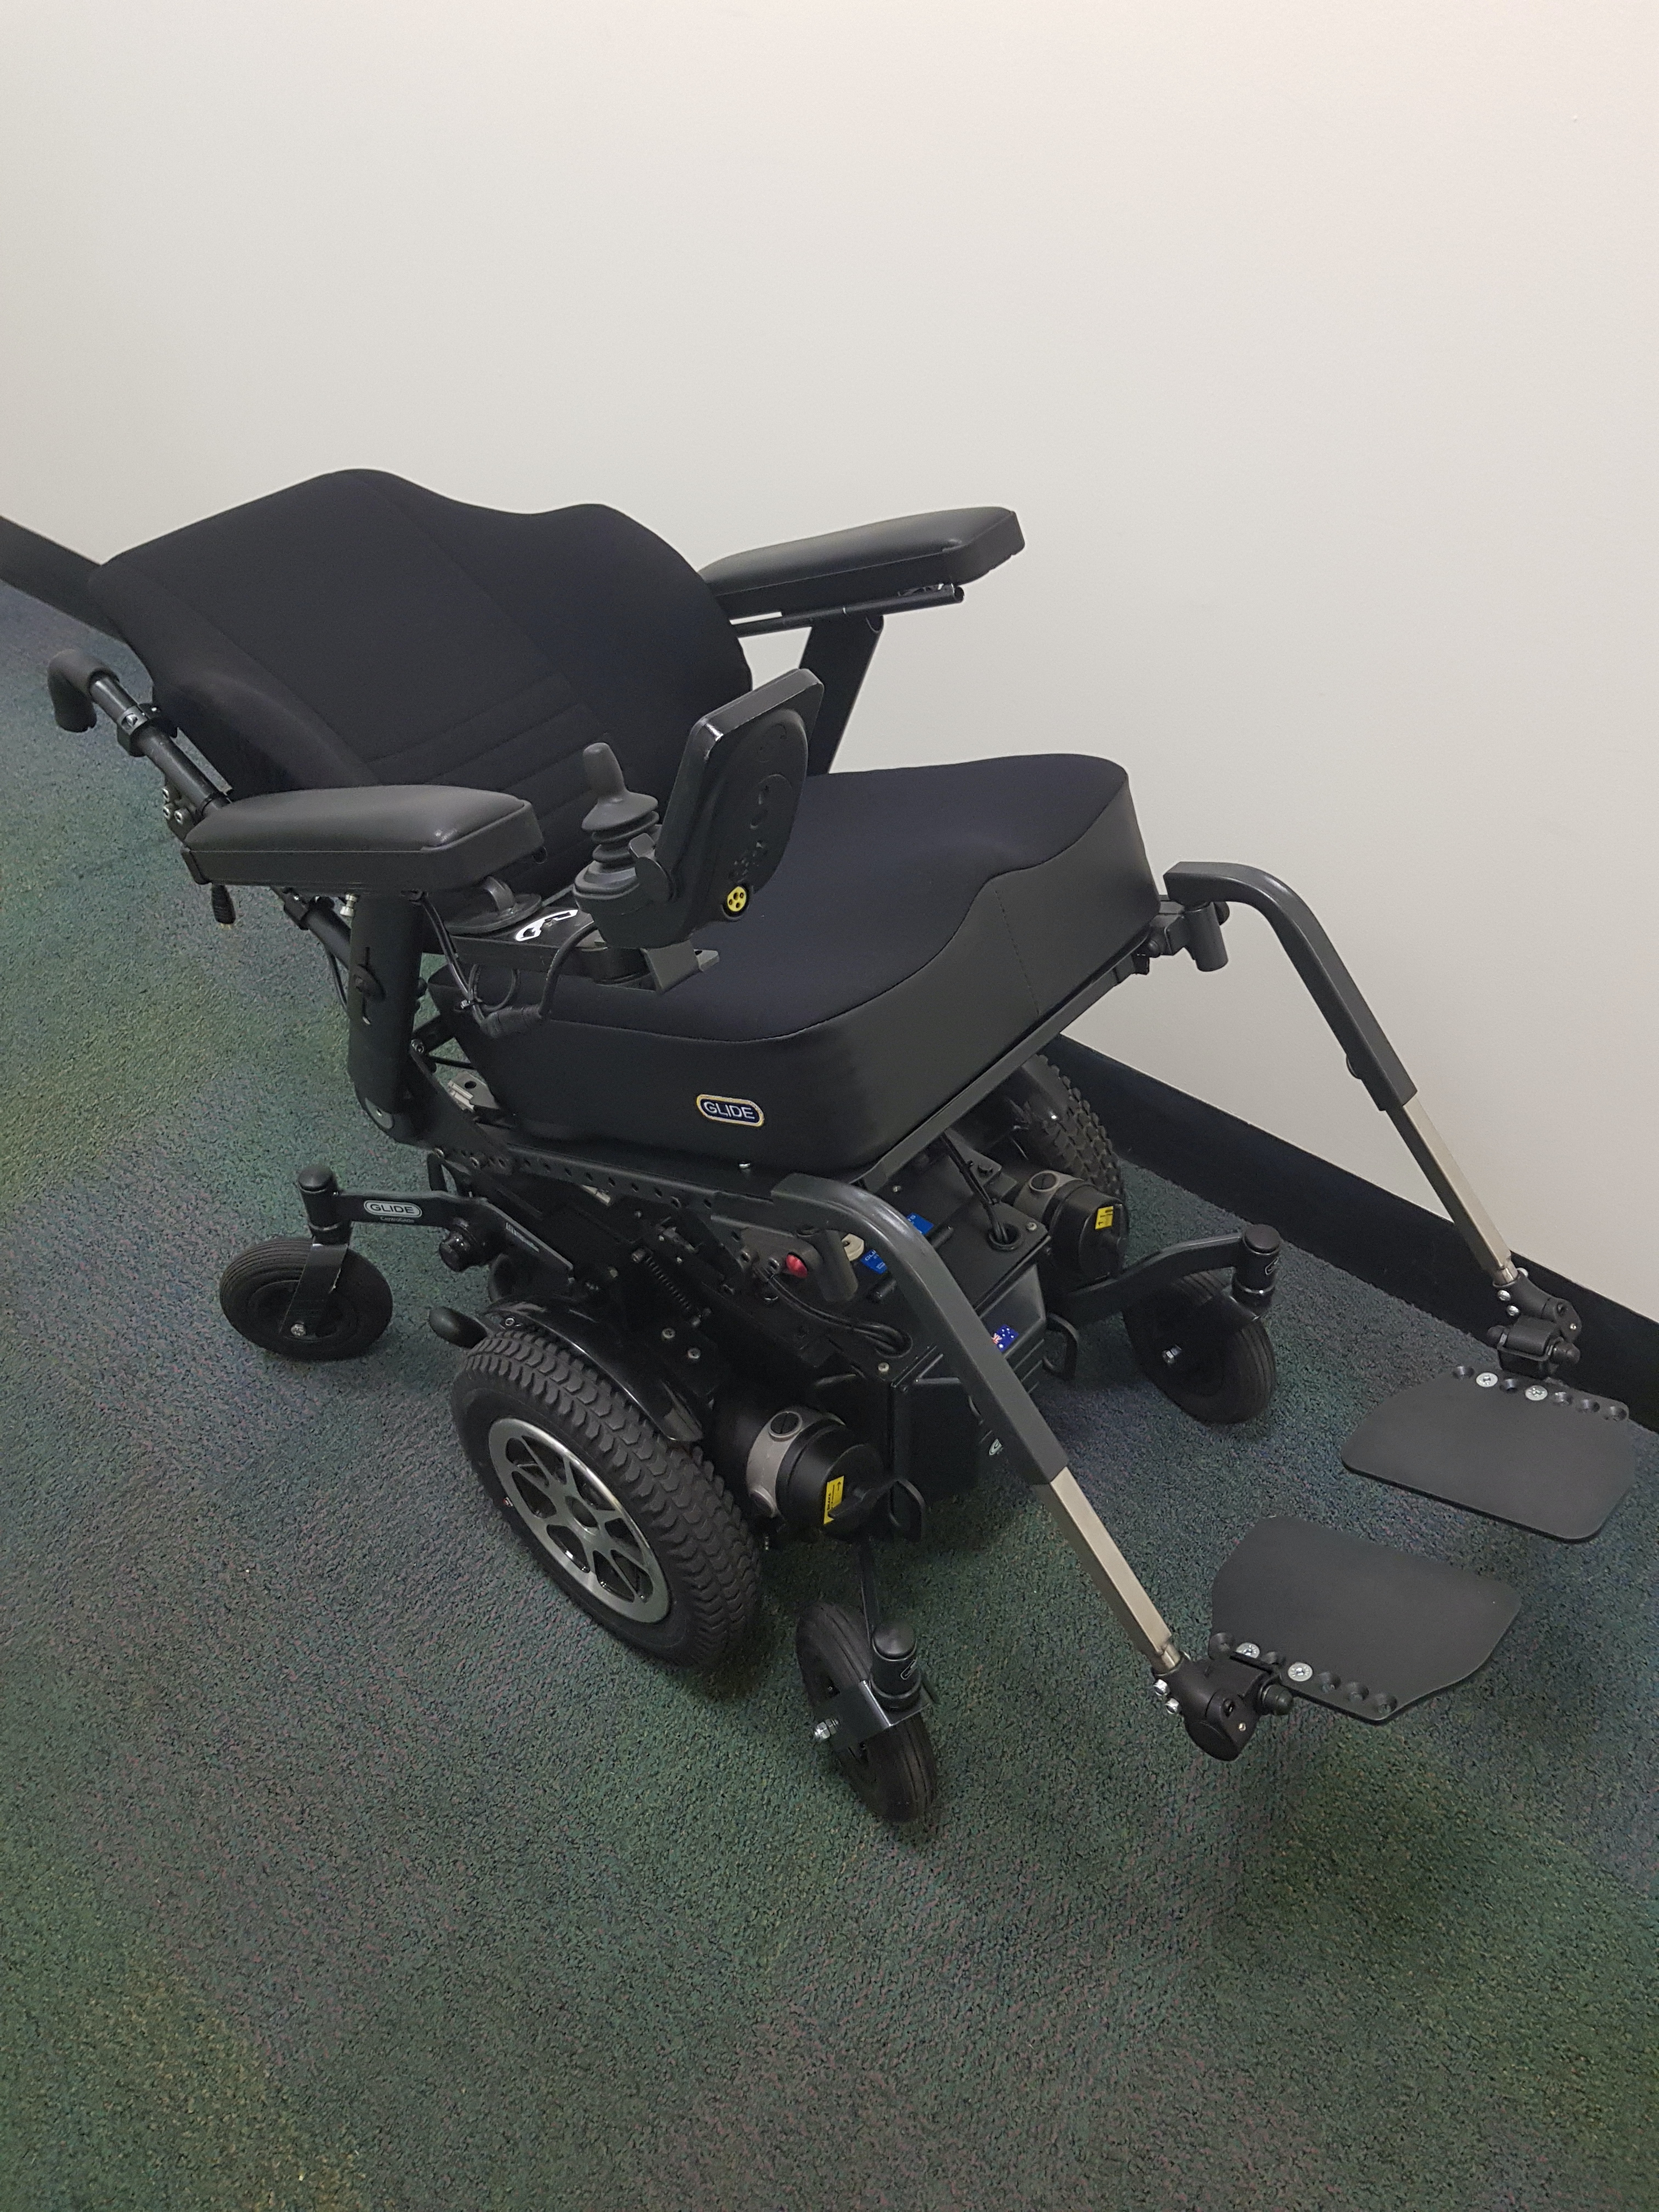
\includegraphics[width=0.4\linewidth]{images/wheelchair_reclined.jpg}
    \caption{CentroGlide wheelchair in reclined position}
    \label{fig:wheelchair_reclined}
\end{figure}
